% ============================================================
% Question Bank: ch06-05 Cross-Sections of Three-Dimensional Figures
% Topic Title: Cross-Sections of Three-Dimensional Figures
% CCSS: 7.G.A.3
% Questions: 30 (18 MC + 7 SA + 5 Graphical)
% ============================================================

% --- Multiple Choice Questions (18) ---

\begin{practiceQuestion}{6-5-q01}{mc}
\begin{questionText}
You slice a rectangular prism with a cut parallel to its base. What shape is the cross-section?
\end{questionText}
\choiceA{Triangle}
\choiceB{Circle}
\choiceC{Rectangle}
\choiceD{Pentagon}
\correctAnswer{C}
\explanation{A horizontal cut parallel to the base of a rectangular prism produces a rectangle the same shape as the base.}
\end{practiceQuestion}

\begin{practiceQuestion}{6-5-q02}{mc}
\begin{questionText}
You slice a cylinder with a horizontal cut parallel to its base. What shape is the cross-section?
\end{questionText}
\choiceA{Rectangle}
\choiceB{Circle}
\choiceC{Oval}
\choiceD{Triangle}
\correctAnswer{B}
\explanation{A horizontal cut through a cylinder parallel to the circular base produces a circle.}
\end{practiceQuestion}

\begin{practiceQuestion}{6-5-q03}{mc}
\begin{questionText}
You slice a cone with a horizontal cut parallel to its base. What shape is the cross-section?
\end{questionText}
\choiceA{A circle smaller than the base}
\choiceB{A circle the same size as the base}
\choiceC{A triangle}
\choiceD{A rectangle}
\correctAnswer{A}
\explanation{A horizontal cut through a cone parallel to the base produces a circle smaller than the base. The higher you cut, the smaller the circle.}
\end{practiceQuestion}

\begin{practiceQuestion}{6-5-q04}{mc}
\begin{questionText}
You slice a sphere with any flat plane. What shape is the cross-section?
\end{questionText}
\choiceA{Oval}
\choiceB{Rectangle}
\choiceC{Circle}
\choiceD{It depends on the angle of the cut}
\correctAnswer{C}
\explanation{Every cross-section of a sphere is a circle. The size of the circle depends on where you cut, but the shape is always a circle.}
\end{practiceQuestion}

\begin{practiceQuestion}{6-5-q05}{mc}
\begin{questionText}
You slice a rectangular pyramid with a cut parallel to the base, halfway up. What shape is the cross-section?
\end{questionText}
\choiceA{A triangle}
\choiceB{A smaller rectangle}
\choiceC{A circle}
\choiceD{A pentagon}
\correctAnswer{B}
\explanation{A horizontal cut parallel to the base of a rectangular pyramid gives a rectangle. It is smaller than the base because the pyramid narrows toward the apex.}
\end{practiceQuestion}

\begin{practiceQuestion}{6-5-q06}{mc}
\begin{questionText}
You slice a cube with a vertical cut from one face to the opposite face, perpendicular to the base. What is the most likely cross-section shape?
\end{questionText}
\choiceA{Square or rectangle}
\choiceB{Circle}
\choiceC{Triangle}
\choiceD{Hexagon}
\correctAnswer{A}
\explanation{A vertical cut through a cube perpendicular to the base typically produces a rectangle. If the cut goes through the center parallel to a face, it can be a square.}
\end{practiceQuestion}

\begin{practiceQuestion}{6-5-q07}{mc}
\begin{questionText}
A triangular prism is sliced with a cut parallel to its triangular base. What is the cross-section?
\end{questionText}
\choiceA{A rectangle}
\choiceB{A triangle congruent to the base}
\choiceC{A smaller triangle}
\choiceD{A trapezoid}
\correctAnswer{B}
\explanation{A cut parallel to the base of a prism always produces a shape congruent (same size and shape) to the base. For a triangular prism, this is a triangle identical to the base.}
\end{practiceQuestion}

\begin{practiceQuestion}{6-5-q08}{mc}
\begin{questionText}
A cylinder is sliced with a vertical cut through its center, perpendicular to the base. What shape is the cross-section?
\end{questionText}
\choiceA{Circle}
\choiceB{Rectangle}
\choiceC{Oval}
\choiceD{Triangle}
\correctAnswer{B}
\explanation{A vertical cut through the center of a cylinder produces a rectangle. The width equals the diameter and the height equals the cylinder's height.}
\end{practiceQuestion}

\begin{practiceQuestion}{6-5-q09}{mc}
\begin{questionText}
You cut a cone with a vertical slice through its apex (tip). What shape is the cross-section?
\end{questionText}
\choiceA{Circle}
\choiceB{Triangle}
\choiceC{Rectangle}
\choiceD{Semicircle}
\correctAnswer{B}
\explanation{A vertical cut through the apex of a cone produces a triangle (specifically an isosceles triangle).}
\end{practiceQuestion}

\begin{practiceQuestion}{6-5-q10}{mc}
\begin{questionText}
A cube can be sliced to produce a hexagonal cross-section. How?
\end{questionText}
\choiceA{By cutting parallel to the base}
\choiceB{By cutting diagonally through all six faces}
\choiceC{By cutting vertically through the center}
\choiceD{It is impossible to get a hexagon from a cube}
\correctAnswer{B}
\explanation{A diagonal plane that passes through all six faces of a cube creates a regular hexagonal cross-section.}
\end{practiceQuestion}

\begin{practiceQuestion}{6-5-q11}{mc}
\begin{questionText}
Which 3D figure always has circular cross-sections when cut parallel to its base?
\end{questionText}
\choiceA{Rectangular prism}
\choiceB{Triangular pyramid}
\choiceC{Cone}
\choiceD{Cube}
\correctAnswer{C}
\explanation{A cone has a circular base, and all horizontal cuts parallel to the base produce circles of varying sizes.}
\end{practiceQuestion}

\begin{practiceQuestion}{6-5-q12}{mc}
\begin{questionText}
A rectangular prism is sliced with a diagonal cut from one edge of the top to the opposite edge of the bottom. What is a possible cross-section?
\end{questionText}
\choiceA{Circle}
\choiceB{Triangle}
\choiceC{Hexagon}
\choiceD{Rectangle}
\correctAnswer{D}
\explanation{A diagonal slice through a rectangular prism from edge to edge can produce a rectangle (or a parallelogram, depending on the angle). A diagonal from top edge to opposite bottom edge typically gives a rectangle.}
\end{practiceQuestion}

\begin{practiceQuestion}{6-5-q13}{mc}
\begin{questionText}
A hexagonal prism is sliced parallel to its base. What is the cross-section?
\end{questionText}
\choiceA{Rectangle}
\choiceB{Triangle}
\choiceC{Hexagon}
\choiceD{Circle}
\correctAnswer{C}
\explanation{Any cut parallel to the base of a prism gives a shape congruent to the base. A hexagonal prism has a hexagonal base, so the cross-section is a hexagon.}
\end{practiceQuestion}

\begin{practiceQuestion}{6-5-q14}{mc}
\begin{questionText}
Which cross-section is NOT possible from slicing a rectangular prism?
\end{questionText}
\choiceA{Rectangle}
\choiceB{Triangle}
\choiceC{Circle}
\choiceD{Pentagon}
\correctAnswer{C}
\explanation{A rectangular prism has flat faces and straight edges. Its cross-sections can be triangles, rectangles, pentagons, or hexagons, but never circles (since it has no curved surfaces).}
\end{practiceQuestion}

\begin{practiceQuestion}{6-5-q15}{mc}
\begin{questionText}
A pyramid with a square base is sliced with a horizontal cut near the top. What shape is the cross-section?
\end{questionText}
\choiceA{A very small square}
\choiceB{A triangle}
\choiceC{A point}
\choiceD{A circle}
\correctAnswer{A}
\explanation{A horizontal cut of a square pyramid parallel to the base gives a square. Near the top, the square is very small. At the very apex it would be a point, but a cut ``near the top'' gives a small square.}
\end{practiceQuestion}

\begin{practiceQuestion}{6-5-q16}{mc}
\begin{questionText}
Which statement about cross-sections is true?
\end{questionText}
\choiceA{The cross-section of any 3D figure is always a circle}
\choiceB{The cross-section depends on the angle and position of the cut}
\choiceC{A cross-section is always the same shape as the base}
\choiceD{Only prisms can have cross-sections}
\correctAnswer{B}
\explanation{The shape of a cross-section depends on where you cut and at what angle. Different cuts through the same figure can produce different shapes.}
\end{practiceQuestion}

\begin{practiceQuestion}{6-5-q17}{mc}
\begin{questionText}
A triangular prism is sliced with a vertical cut perpendicular to the triangular bases. What shape is the cross-section?
\end{questionText}
\choiceA{Triangle}
\choiceB{Rectangle}
\choiceC{Circle}
\choiceD{Trapezoid}
\correctAnswer{B}
\explanation{A vertical cut perpendicular to the triangular bases of a triangular prism produces a rectangle (the cut goes through the lateral faces).}
\end{practiceQuestion}

\begin{practiceQuestion}{6-5-q18}{mc}
\begin{questionText}
You cut a rectangular prism with a cut that passes through exactly three faces. What is the cross-section shape?
\end{questionText}
\choiceA{Rectangle}
\choiceB{Triangle}
\choiceC{Pentagon}
\choiceD{Hexagon}
\correctAnswer{B}
\explanation{A plane that intersects exactly three faces of a rectangular prism creates a triangular cross-section (one edge on each of the three faces).}
\end{practiceQuestion}

% --- Short Answer Questions (7) ---

\begin{practiceQuestion}{6-5-q19}{sa}
\begin{questionText}
What shape is the cross-section when you cut a sphere through its center?
\end{questionText}
\correctAnswer{A circle (the largest possible circle)}
\explanation{A cut through the center of a sphere produces a great circle — the largest possible circular cross-section, with the same radius as the sphere.}
\end{practiceQuestion}

\begin{practiceQuestion}{6-5-q20}{sa}
\begin{questionText}
A rectangular prism has a base of $6$ cm by $4$ cm and a height of $10$ cm. It is sliced parallel to the base. What are the dimensions of the cross-section?
\end{questionText}
\correctAnswer{$6$ cm by $4$ cm}
\explanation{A cut parallel to the base of a rectangular prism produces a rectangle identical to the base: $6$ cm by $4$ cm.}
\end{practiceQuestion}

\begin{practiceQuestion}{6-5-q21}{sa}
\begin{questionText}
What shape is the cross-section when a cone is sliced vertically through its apex?
\end{questionText}
\correctAnswer{A triangle}
\explanation{A vertical slice through the apex of a cone produces an isosceles triangle. The base of the triangle is a diameter of the cone's base.}
\end{practiceQuestion}

\begin{practiceQuestion}{6-5-q22}{sa}
\begin{questionText}
Name two different cross-section shapes you can get from slicing a cube.
\end{questionText}
\correctAnswer{Any two of: square, rectangle, triangle, pentagon, hexagon}
\explanation{A cube can be sliced to produce squares, rectangles, triangles, pentagons, or hexagons depending on the angle and position of the cut.}
\end{practiceQuestion}

\begin{practiceQuestion}{6-5-q23}{sa}
\begin{questionText}
A cylinder has a radius of $5$ cm and height of $12$ cm. It is sliced vertically through its center. What shape is the cross-section and what are its dimensions?
\end{questionText}
\correctAnswer{Rectangle; $10$ cm by $12$ cm}
\explanation{A vertical cut through the center of a cylinder produces a rectangle. Width = diameter = $2 \times 5 = 10$ cm. Height = $12$ cm.}
\end{practiceQuestion}

\begin{practiceQuestion}{6-5-q24}{sa}
\begin{questionText}
Is it possible to get a circular cross-section from a rectangular prism? Explain.
\end{questionText}
\correctAnswer{No}
\explanation{A rectangular prism has only flat faces and straight edges. All cross-sections are polygons (triangles, rectangles, pentagons, hexagons). A circular cross-section requires a curved surface.}
\end{practiceQuestion}

\begin{practiceQuestion}{6-5-q25}{sa}
\begin{questionText}
A square pyramid has a base edge of $8$ cm. It is sliced parallel to the base halfway up. Is the cross-section larger, smaller, or the same size as the base?
\end{questionText}
\correctAnswer{Smaller than the base}
\explanation{A horizontal cut parallel to the base of a pyramid produces a similar shape that is smaller than the base. Halfway up, the cross-section is a $4$ cm square (half the edge length).}
\end{practiceQuestion}

% --- Graphical Questions (3 GMC + 2 GSA) ---

\begin{practiceQuestion}{6-5-q26}{gmc}
\begin{questionText}
The diagram shows a rectangular prism being sliced by a horizontal plane (dashed line). What is the cross-section?

\begin{center}
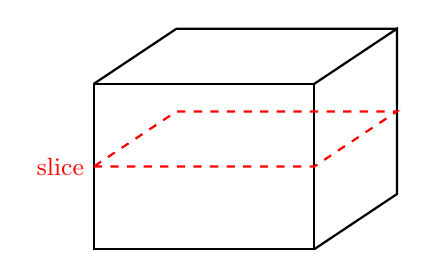
\begin{tikzpicture}[scale=0.7]
  % Rectangular prism
  \draw[thick] (0,0) -- (4,0) -- (4,3) -- (0,3) -- cycle; % front face
  \draw[thick] (4,0) -- (5.5,1) -- (5.5,4) -- (4,3); % right face
  \draw[thick] (0,3) -- (1.5,4) -- (5.5,4); % top face
  \draw[dashed,thick,red] (0,1.5) -- (4,1.5) -- (5.5,2.5) -- (1.5,2.5) -- cycle;
  \node[left,red] at (0,1.5) {\small slice};
\end{tikzpicture}
\end{center}
\end{questionText}
\choiceA{Triangle}
\choiceB{Rectangle}
\choiceC{Circle}
\choiceD{Trapezoid}
\correctAnswer{B}
\explanation{A horizontal slice through a rectangular prism always produces a rectangle congruent to the base.}
\end{practiceQuestion}

\begin{practiceQuestion}{6-5-q27}{gmc}
\begin{questionText}
The diagram shows a cone being sliced. Which cut produces a circular cross-section?

\begin{center}
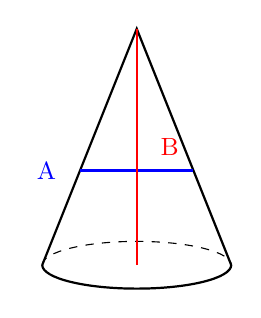
\begin{tikzpicture}[scale=0.6]
  % Cone
  \draw[thick] (-2,0) -- (0,5) -- (2,0);
  \draw[thick] (-2,0) arc[start angle=180,end angle=360,x radius=2,y radius=0.5];
  \draw[dashed] (-2,0) arc[start angle=180,end angle=0,x radius=2,y radius=0.5];
  % Cut A - horizontal
  \draw[thick,blue] (-1.2,2) -- (1.2,2);
  \node[left,blue] at (-1.5,2) {\small A};
  % Cut B - vertical through apex
  \draw[thick,red] (0,0) -- (0,5);
  \node[right,red] at (0.3,2.5) {\small B};
\end{tikzpicture}
\end{center}
\end{questionText}
\choiceA{Cut A (horizontal)}
\choiceB{Cut B (vertical through apex)}
\choiceC{Both cuts}
\choiceD{Neither cut}
\correctAnswer{A}
\explanation{Cut A (horizontal, parallel to the base) produces a circle. Cut B (vertical through the apex) produces a triangle.}
\end{practiceQuestion}

\begin{practiceQuestion}{6-5-q28}{gmc}
\begin{questionText}
The diagram shows a triangular prism. A cut is made parallel to the triangular base (shown as the shaded region). What is the cross-section?

\begin{center}
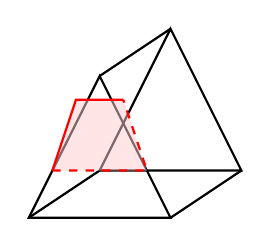
\begin{tikzpicture}[scale=0.6]
  % Front triangle
  \draw[thick] (0,0) -- (3,0) -- (1.5,3) -- cycle;
  % Back triangle
  \draw[thick] (1.5,1) -- (4.5,1) -- (3,4) -- cycle;
  % Connecting edges
  \draw[thick] (0,0) -- (1.5,1);
  \draw[thick] (3,0) -- (4.5,1);
  \draw[thick] (1.5,3) -- (3,4);
  % Cross section
  \fill[red!20,opacity=0.5] (0.5,1) -- (2.5,1) -- (2,2.5) -- (1,2.5) -- cycle;
  \draw[thick,red,dashed] (0.5,1) -- (2.5,1) -- (2,2.5);
  \draw[thick,red] (0.5,1) -- (1,2.5) -- (2,2.5);
\end{tikzpicture}
\end{center}
\end{questionText}
\choiceA{Rectangle}
\choiceB{Triangle}
\choiceC{Circle}
\choiceD{Hexagon}
\correctAnswer{B}
\explanation{A cut parallel to the base of a prism gives a shape congruent to the base. Since the base is a triangle, the cross-section is a triangle.}
\end{practiceQuestion}

\begin{practiceQuestion}{6-5-q29}{gsa}
\begin{questionText}
The diagram shows a cylinder with radius $4$ cm and height $9$ cm. A vertical cut is made through the center. Describe the cross-section and give its dimensions.

\begin{center}
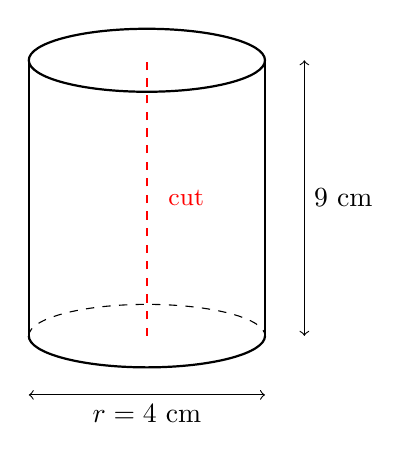
\begin{tikzpicture}[scale=0.5]
  % Cylinder
  \draw[thick] (-3,0) -- (-3,7);
  \draw[thick] (3,0) -- (3,7);
  \draw[thick] (-3,0) arc[start angle=180,end angle=360,x radius=3,y radius=0.8];
  \draw[dashed] (-3,0) arc[start angle=180,end angle=0,x radius=3,y radius=0.8];
  \draw[thick] (-3,7) arc[start angle=180,end angle=360,x radius=3,y radius=0.8];
  \draw[thick] (-3,7) arc[start angle=180,end angle=0,x radius=3,y radius=0.8];
  % Vertical cut line
  \draw[thick,red,dashed] (0,0) -- (0,7);
  \node[right,red] at (0.3,3.5) {\small cut};
  % Labels
  \draw[<->] (-3,-1.5) -- (3,-1.5);
  \node[below] at (0,-1.5) {$r = 4$ cm};
  \draw[<->] (4,0) -- (4,7);
  \node[right] at (4,3.5) {$9$ cm};
\end{tikzpicture}
\end{center}
\end{questionText}
\correctAnswer{Rectangle; $8$ cm by $9$ cm}
\explanation{A vertical cut through the center of a cylinder produces a rectangle. Width = diameter = $2 \times 4 = 8$ cm. Height = $9$ cm.}
\end{practiceQuestion}

\begin{practiceQuestion}{6-5-q30}{gsa}
\begin{questionText}
The diagram shows a cube with edge length $6$ cm. A diagonal cut is made from vertex $A$ through the center to the opposite vertex $B$, passing through four faces. What type of shape could this cross-section be?

\begin{center}
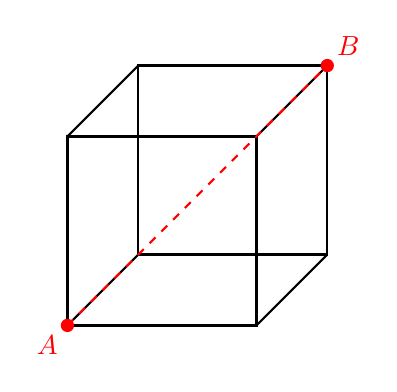
\begin{tikzpicture}[scale=0.6]
  % Front face
  \draw[thick] (0,0) -- (4,0) -- (4,4) -- (0,4) -- cycle;
  % Back face
  \draw[thick] (1.5,1.5) -- (5.5,1.5) -- (5.5,5.5) -- (1.5,5.5) -- cycle;
  % Connecting edges
  \draw[thick] (0,0) -- (1.5,1.5);
  \draw[thick] (4,0) -- (5.5,1.5);
  \draw[thick] (4,4) -- (5.5,5.5);
  \draw[thick] (0,4) -- (1.5,5.5);
  % Diagonal vertices
  \fill[red] (0,0) circle (4pt) node[below left] {$A$};
  \fill[red] (5.5,5.5) circle (4pt) node[above right] {$B$};
  % Diagonal line
  \draw[thick,red,dashed] (0,0) -- (5.5,5.5);
\end{tikzpicture}
\end{center}
\end{questionText}
\correctAnswer{A rectangle}
\explanation{A diagonal cut from one vertex of a cube to the opposite vertex, passing through four faces, creates a rectangular cross-section. The rectangle's dimensions are a face diagonal ($6\sqrt{2}$ cm) by the edge length ($6$ cm).}
\end{practiceQuestion}
